\documentclass[pdftex,12pt,letter]{article}
\usepackage{fancyhdr}
\usepackage{enumerate}
\usepackage{tabularx}
\usepackage{graphicx}
\usepackage{array}
\usepackage[justification=justified,singlelinecheck=false]{caption}
\pagestyle{fancy}
\makeatletter
  \renewcommand\@seccntformat[1]{\csname the#1\endcsname.\quad}
\makeatother

\newcolumntype {Y}{ >{\raggedright \arraybackslash }X}
\newcommand{\HRule}{\rule{\linewidth}{0.5mm}}
\captionsetup{labelformat=empty}

\begin{document}

\begin{titlepage}
\begin{flushright}
\HRule \\[0.4cm]
{ \bfseries
{\huge Software Requirements Specification\\[1cm]}
{\Large for\\[1cm]}
{\huge CWRUtility\large{\footnote[1]{Working title}}\\[4cm]}
{\large Prepared by\\Jason Kuster, Stuart Long, and William Ordivay\\[1cm]
Version 1.0\\[1cm]
KOALAA Development\\[1cm]
October 1, 2012}}
\end{flushright}
\end{titlepage}
\tableofcontents{}
\vspace{5cm}
\begin{table}[h]
\caption*{\bfseries Revision History}
\begin{tabularx}{\textwidth }[t]{|l|Y|Y|Y|}
\hline
\bfseries Name & \bfseries Date & \bfseries Reasons for Change & \bfseries Version \\ \hline
Kuster, Long, Ordiway & 9/22/2012 & Initial Draft & 1.0 draft 1\\ \hline
\end{tabularx}
\end{table}
\newpage
\section{Introduction}
\subsection{Purpose}
This Software Requirements Specification describes the software functional and nonfunctional requirements for release 1.0 of CWRUtility. This specification document is intended for the solu use of the members of the project team that will implement and verify the correction functioning of the system. Unless otherwise specified, all requirements documented here are high priority and committed for release 1.0. 

\subsection{Project Scope and Product Features}
CWRUtility will allow CWRU students, faculty, and staff to easily access CWRU services and information in an easy-to-use way. A detailed project description is available in the \emph{CWRUTility Vision and Scope Document}[1]. The section in that document titled "Scope of initial and subsequent releases" lists the features that are scheduled for full or partial implementation in this release.

\subsection{Business Risks}
\begin{enumerate}[BR-1:]
\item Application fails certification for the Windows Phone Store.
\item Windows Phone is a currently less utilized application platform than its competitors, increasing the risk that fewer students will use the application.
\end{enumerate}

\section{Overall Description}
\subsection{Product Perspective}
CWRUtility is a new system that replaces the need for cumbersome navigation of all of the CWRU services in favor of a streamlined and custom-built mobile experience. The context diagram in Figure 1 illustrates the external entities and system interfaces for release 1.0. The system is expected to evolve over two releases, ultimately encompassing all of the services CWRU students, faculty, and staff use every day.
\subsection{User Classes and Characteristics}
CWRUtility Users: CWRUtility users are CWRU students, faculty, or staff members who wish to use our app in order to access CWRU services. The number of people at CWRU who possess Windows Phone 7/8 devices is is unknown, but can be estimated in the area of 200 to 400 assuming that about half to 3/4 of the community possesses smartphones and the current figures put Windows Phone's marketshare at 3.5\%. Our app will probably be used daily by 75\% of installed users.\\
CWRU Services:  The CWRU services are the services enumerated in Diagram 1 with which CWRUtility will have active communication. These services will be accessed several times per day by each instance of the application as it pulls data from the background. Multiple users may access the same service at the same time. Downtime in a service will result in downtime for the application.
\subsection{Assumptions and Dependencies}
\begin{enumerate}[{A}S-1:]
\item Mobile device is equipped with an internet connection.
\end{enumerate}
\begin{enumerate}[DE-1:]
\item This application depends on the continuing functionality of the described services.
\end{enumerate}
\section{Scope and Limitations}
\subsection{Scope of Initial and Subsequent Releases}
\begin{table}[h]
\begin{tabularx}{\textwidth }[t]{|l|Y|Y|Y|}
\hline
\bfseries Feature & \bfseries\hspace{1cm}Release 1 & \bfseries\hspace{1cm}Release 2 & \bfseries\hspace{1cm}Release 3 \\ \hline
FE-1 & Fully implemented & ~ & ~ \\ \hline
FE-2 & Basic map & Integrated with course schedule & Provides directions \\ \hline
FE-3 & Basic functionality with NextBus & Full integration with NextBus (if needed) & Integration with Map \\ \hline
FE-4 & Fully implemented & ~ & ~ \\ \hline
FE-5 & Not implemented & Fully implemented & ~ \\ \hline
FE-6 & Fully implemented & ~ & ~ \\ \hline
FE-7 & Not implemented & Fully implemented & ~ \\ \hline
FE-8 & Not implemented & Basic information displays & Integrates with phone's notification system \\ \hline
FE-9 & Table of events & ~ & Integrated with course schedule \\ \hline
FE-10 & Not implemented & Fully implemented & ~ \\
\hline
\end{tabularx}
\end{table}
\subsection{Limitations and Exclusions}
\begin{enumerate}[L{I}-1:]
\item Requires functioning internet connection.
\item Dependency on external services.
\end{enumerate}
\begin{enumerate}[EX-1:]
\item Available only for Windows Phone 7 / Windows Phone 8 mobile devices.
\end{enumerate}
\section{Business Context}
\subsection{User Profile}
\begin{table}[h]
\begin{tabularx}{\textwidth}[t]{|Y|Y|Y|Y|}
\hline
\bfseries User & \bfseries Value & \bfseries Interests & \bfseries Constraints\\ \hline
CWRU community members & More efficient and centralized use of CWRU services and resources & Ease of use; reliability; simplicity & Required to have a Windows Phone 7/8 with internet access \\ \hline
CWRU service providers & increased discoverability and utilization of their services & Appropriate representation of services in software & Potential for communication with CWRUtility to malfunction after service updates \\ \hline
\end{tabularx}
\end{table}

\lfoot{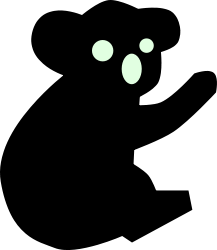
\includegraphics[height=1cm]{DarkKoala.png}}
\end{document}